\documentclass[12pt,letterpaper]{article}
\usepackage[utf8]{inputenc}
\usepackage[spanish]{babel}
\usepackage{graphicx}
\usepackage[left=2cm,right=2cm,top=2cm,bottom=2cm]{geometry}
\usepackage{graphicx} % figuras
\usepackage{hyperref}
% \usepackage{subfigure} % subfiguras
\usepackage{float} % para usar [H]
\usepackage{amsmath}
%\usepackage{txfonts}
\usepackage{stackrel} 
\usepackage{multirow}
\usepackage{enumerate} % enumerados
\renewcommand{\labelitemi}{$-$}
\renewcommand{\labelitemii}{$\cdot$}
% \author{}
% \title{Caratula}
\begin{document}

% Fancy Header and Footer
% \usepackage{fancyhdr}
% \pagestyle{fancy}
% \cfoot{}
% \rfoot{\thepage}
%

% \usepackage[hidelinks]{hyperref} % CREA HYPERVINCULOS EN INDICE

% \author{}
\title{Caratula}

\begin{titlepage}
\begin{center}
\large{UNIVERSIDAD PRIVADA-DE-TACNA}\\
\vspace*{-0.025in}
\begin{figure}[htb]
\begin{center}

\includegraphics[width=8cm]{./Imagenes/logo}
\end{center}
\end{figure}
\vspace*{0.15in}
INGENIERIA DE SISTEMAS  \\

\vspace*{0.5in}
\begin{large}
TITULO:\\
\end{large}

\vspace*{0.1in}
\begin{Large}
\textbf{INFORME DE LABORATORIO No 04} \\
\end{Large}

\vspace*{0.3in}
\begin{Large}
\textbf{CURSO:} \\
\end{Large}

\vspace*{0.1in}
\begin{large}
INTELIGENCIA DE NEGOCIOS\\
\end{large}

\vspace*{0.3in}
\begin{Large}
\textbf{DOCENTE(ING):} \\
\end{Large}

\vspace*{0.1in}
\begin{large}
 Patrick Cuadros Quiroga\\
\end{large}

\vspace*{0.2in}
\vspace*{0.1in}
\begin{large}
Integrante: \\
\begin{flushleft}
Arlyn Alejandra Cotrado Coaquira	\hfill	(2016054466) 
\end{flushleft}
\end{large}
\end{center}

\end{titlepage}



\thispagestyle{empty} % INDICE SIN NUMERO
\newpage
\setcounter{page}{1} % REINICIAR CONTADOR DE PAGINAS DESPUES DEL INDICE


\section{DESARROLLO}
\subsection{Ejercicio N01: Envios}

\begin{itemize}
\item  
	\begin{center}
	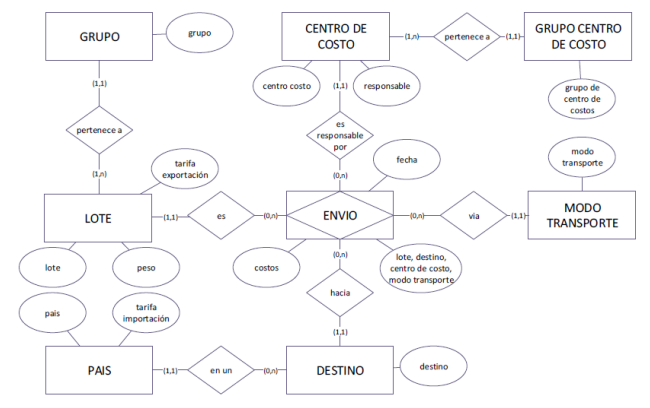
\includegraphics[width=14cm]{./Imagenes/e1}
	\end{center}
	\item Su modelo dimensional:
	\begin{center}
	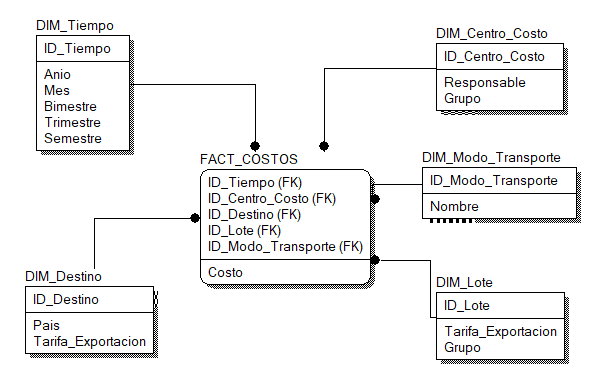
\includegraphics[width=14cm]{./Imagenes/d1}
	\end{center}
\item Su script:
	\begin{center}
	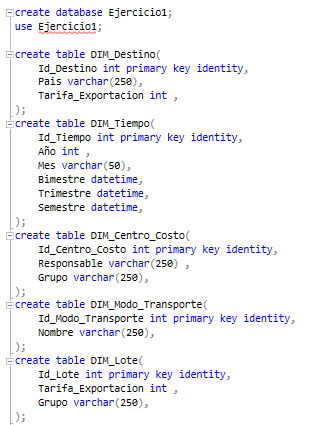
\includegraphics[width=8cm]{./Imagenes/s1-1}
	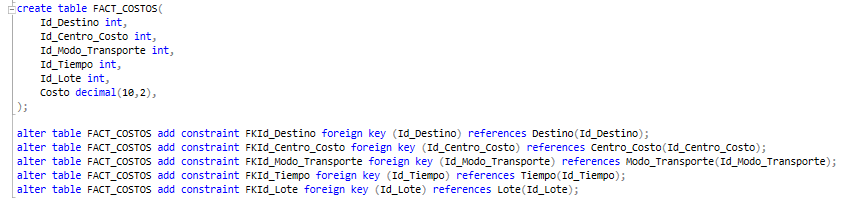
\includegraphics[width=14cm]{./Imagenes/s1-2}
	\end{center}

\end{itemize}

\subsection{ Ejercicio N02: Reservas de viaje}
\begin{itemize}
\item  
	\begin{center}
	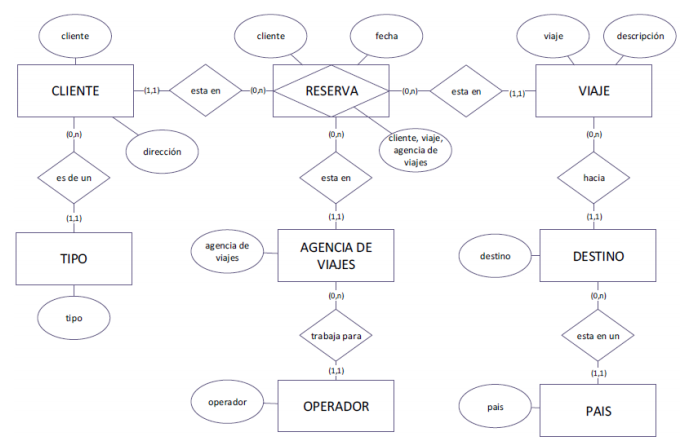
\includegraphics[width=14cm]{./Imagenes/e2}
	\end{center}
	\item Su modelo dimensional:
	\begin{center}
	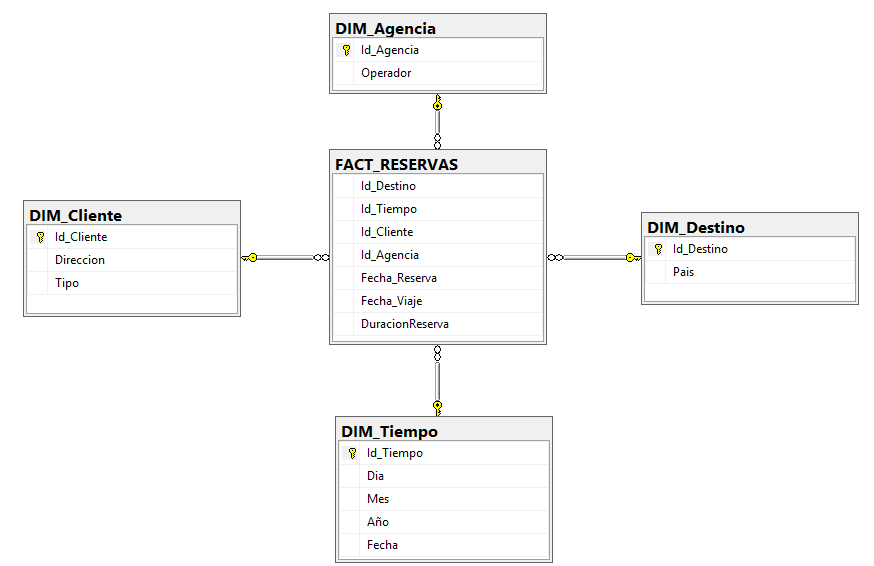
\includegraphics[width=14cm]{./Imagenes/d2}
	\end{center}
\item Su script:
	\begin{center}
	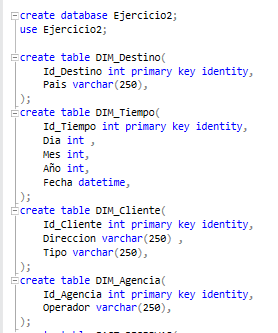
\includegraphics[width=8cm]{./Imagenes/s2-1}
	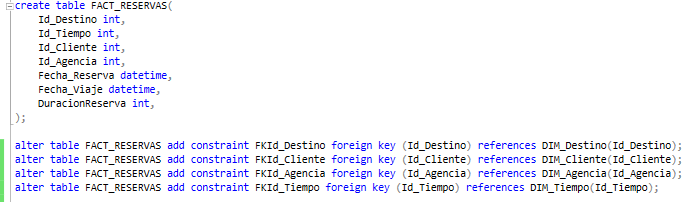
\includegraphics[width=14cm]{./Imagenes/s2-2}
	\end{center}

\end{itemize}

\subsection{ Ejercicio N02: Gestión de proyectos}

\begin{itemize}
\item  
	\begin{center}
	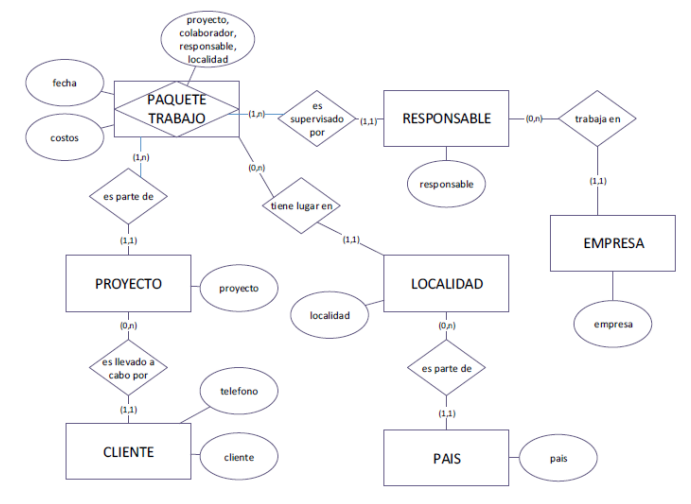
\includegraphics[width=14cm]{./Imagenes/e3}
	\end{center}
	\item Su modelo dimensional:
	\begin{center}
	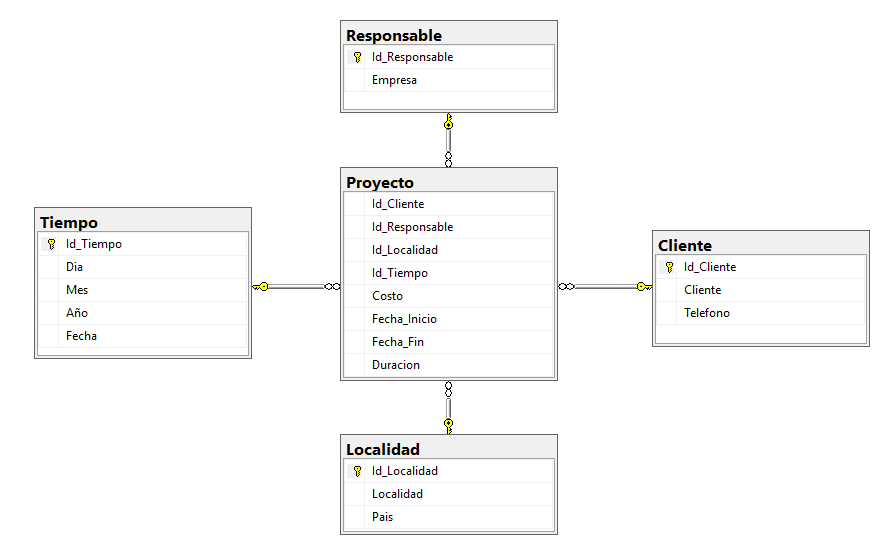
\includegraphics[width=14cm]{./Imagenes/d3}
	\end{center}
\item Su script:
	\begin{center}
	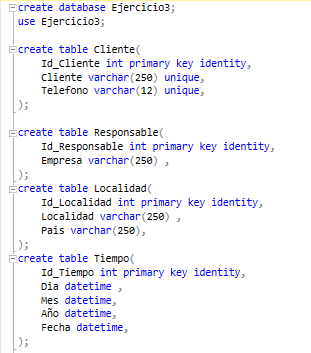
\includegraphics[width=8cm]{./Imagenes/s3-1}
	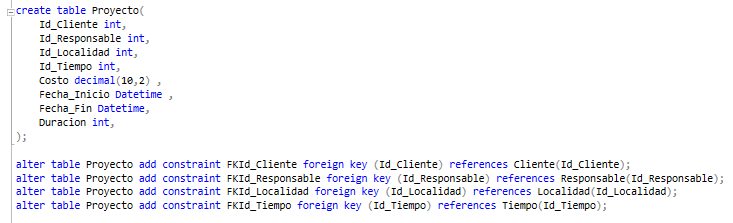
\includegraphics[width=14cm]{./Imagenes/s3-2}
	\end{center}

\end{itemize}

\end{document}
